\chapter{The workshop: twenty contest problems}\label{ch:workshop}

Part mechanics, part method: twenty original problems that deliberately
mix chapters --- energy plus rolling, Faraday plus momentum. Each comes
with a hint (one line, for the stuck) and a full solution in the
\emph{Strategy}$\to$\emph{Solution}$\to$\emph{Significance} frame the
rest of the book uses.

\section{Contest method in one page}\label{sec:ws-method}

\begin{itemize}
\item \textbf{Units first}: any answer failing dimensional analysis is
wrong before it is checked.
\item \textbf{Limits before algebra}: $m\to0$, $\mu\to0$, $r\to\infty$
--- every formula you write should survive its limits.
\item \textbf{Conservation before integration}: check $p$, $L$, $E$
conservation \emph{first}; integrate only when forced.
\item \textbf{Audit, then trust}: every solution ends with a number you
can sanity-check against an order of magnitude.
\end{itemize}

\section{The problems}\label{sec:ws-problems}

\begin{description}
\item[W1] (medium; F=ma-style) A ball is thrown at $20$\,m/s; its
terminal speed is $33$\,m/s. What fraction of its weight is the drag at
launch? When does drag actually matter?
\item[W2] (medium; F=ma) A $3$\,kg block on a table ($\mu_s=0.4$,
$\mu_k=0.3$) ties over a pulley to a hanging mass. Find the largest
hanging mass that never moves, and the acceleration when it hangs
$2$\,kg instead.
\item[W3] (medium; F=ma) Ball A rolls at $2$\,m/s and hits identical
ball B elastically; B leaves a $1.25$\,m table and lands $1$\,m out.
Are the numbers consistent with a clean hit?
\item[W4] (medium; AP-C) A $1$\,kg ball at $2$\,m/s hits a stationary
$2$\,kg ball with $e=0.5$. Find both final speeds and audit the lost
energy.
\item[W5] (hard; APhO-style) A spool of outer radius $R$, inner $r$
rests on a table; a thread wound on the inner radius is pulled at
angle $\theta$ above horizontal. Which way does it roll?
\item[W6] (medium; F=ma data) A meter stick pivots about its $20$\,cm
mark. Find its small-oscillation period.
\item[W7] (medium; F=ma) A satellite in a circular $1.5R_E$ orbit
transfers to $2.5R_E$. Find the two burns and total $\Delta v$.
\item[W8] (hard; USAPhO) A $100$\,kg satellite docks with a spinning
$1000$\,kg station ($I=5000$\,kg\,m$^{2}$) at its $5$\,m rim; the
station spun at $0.5$\,rad/s. Find the new rate.
\item[W9] (hard; USAPhO classic) A frictionless tunnel runs straight
through a uniform-density Earth. Show the transit time to the far side
and explain why it does not depend on where the tunnel runs.
\item[W10] (hard; APhO) A $50$\,kg cart rolls at $5$\,m/s while sand
rains in vertically at $2$\,kg/s. Find $v(t)$ and explain the missing
force.
\item[W11] (medium; AP-C FR) Find the field on the axis of a uniformly
charged disk at height $z$; take the $z\gg R$ limit.
\item[W12] (hard; USAPhO) A point charge sits off-centre inside a
conducting shell's cavity. Find the charges induced on each surface
and argue the exterior field's shape.
\item[W13] (medium; F=ma) Two $10$\,g balls each with charge
$+1$\,\textmu C are released $10$\,cm apart. Speed when far apart?
\item[W14] (hard; APhO) A dielectric slab slides part-way into a
charged, \emph{isolated} capacitor. Find the work done by the field
pulling it in, and where the energy went.
\item[W15] (medium; F=ma data) A $10$\,k$\Omega$ voltmeter measures
across the $5$\,k$\Omega$ lower leg of a $10\text{k}\!+\!5$\,k divider
on $15$\,V. What does it read?
\item[W16] (hard; USAPhO) Charging a capacitor through a resistor
always dissipates half the battery's energy --- independent of $R$.
Where did it go? Resolve the ``paradox'' for $R\to0$.
\item[W17] (medium; AP-C FR) Design a velocity selector passing
$3\times10^{5}$\,m/s ions through a $0.01$\,T field.
\item[W18] (hard; USAPhO classic) A rod slides down vertical
frictionless rails joined by resistor $R$ in field $B$. Find its
terminal velocity and audit the powers.
\item[W19] (medium; AP-C) An RLC circuit rings at the same frequency as
a familiar mechanical oscillator. State both frequencies.
\item[W20] (hard; estimation) Deliver $1$\,kW to a $12$\,V load over
$0.5\,\Omega$ of line. Compare raw versus stepped-up:
estimate the loss reduction.
\end{description}

\section{Hints}\label{sec:ws-hints}

\begin{description}
\item[W1] Drag $\propto v^{2}$; at terminal it equals $mg$.
\item[W2] Static friction supplies up to $\mu_sN$ --- check the
boundary first.
\item[W3] Equal-mass elastic = swap; then free-fall from the table.
\item[W4] $v_1'=v_1(1-e)/\text{...}$ --- use the restitution formulas;
loss $\propto(1-e^{2})$.
\item[W5] Torque about the contact point: $F(R\cos\theta-r)$.
\item[W6] $T=2\pi\sqrt{I/(mgd)}$ with $d$ the pivot--CM distance.
\item[W7] Hohmann: vis-viva at both burns.
\item[W8] Conserve $L$ about the spin axis; $L_{new}=I_{tot}\omega'$.
\item[W9] $g(r)\propto r$ inside a uniform sphere --- that's Hooke's
law.
\item[W10] Sand carries no horizontal momentum: $dP=0$ along the track.
\item[W11] Symmetry leaves only the $z$-component to integrate.
\item[W12] Conductor field zero $\Rightarrow$ inner surface $=-q$;
conservation fixes the outer.
\item[W13] Energy: stored $\to$ kinetic of \emph{both}.
\item[W14] Isolated means $Q$ fixed: $U=Q^{2}/2C$ drops as $C$ grows.
\item[W15] The meter is a parallel resistor: re-compute the divider.
\item[W16] The dissipation is in the resistor \emph{or} the spark ---
either way it isn't in the cap.
\item[W17] $qE=qvB$ when undeflected.
\item[W18] At terminal: gravity power $=$ dissipated power.
\item[W19] $\omega_0=1/\sqrt{LC}$ is chapter~7's $\sqrt{k/m}$ with the
map already made in chapter~14.
\item[W20] $I^{2}R$ scales the wrong way at low $V$: step up first.
\end{description}

\section{Solutions}\label{sec:ws-sol}

\begin{example}[W1: drag bound]\label{ex:w1}
At launch the ball moves at $20$\,m/s with $v_t=33$\,m/s.
\par\smallskip
\textbf{Strategy.} Quadratic drag: $F_D=mg(v/v_t)^{2}$.
\begin{solution}
$F_D/mg=(20/33)^{2}=0.37$: drag is already $37\%$ of weight at launch
--- it matters everywhere for a baseball-speed throw; only
$v\ll v_t/3$ lets you ignore it. \checkmark
\end{solution}
\textbf{Significance.} The ``when does drag matter'' question has a
number: the ratio $(v/v_t)^{2}$, not vibes.
\end{example}

\begin{example}[W2: pulley + friction boundary]\label{ex:w2}
$3$\,kg on the table, $\mu_s=0.4$, $\mu_k=0.3$.
\par\smallskip
\textbf{Strategy.} Static boundary: $m_2g=\mu_sm_1g$.
\begin{solution}
Boundary at $m_2=1.2$\,kg: nothing moves for $m_2\le1.2$\,kg.
With $m_2=2$\,kg sliding:
$a=(2-0.9)g/5=2.16$\,m/s$^{2}$. \checkmark
\end{solution}
\textbf{Significance.} Static/kinetic regimes have different answers;
always find the boundary first.
\end{example}

\begin{example}[W3: collision + projectile consistency]\label{ex:w3}
Does a $2$\,m/s approach give a $1$\,m landing at $1.25$\,m height?
\par\smallskip
\textbf{Strategy.} Elastic equal masses swap velocities; then
projectile time.
\begin{solution}
B takes $2$\,m/s. Fall time $t=\sqrt{2(1.25)/9.8}=0.505$\,s;
range $=2\times0.505=1.01$\,m --- consistent to rounding. \checkmark
\end{solution}
\textbf{Significance.} Two chapters in one problem; the chain is the
point.
\end{example}

\begin{figure}[htbp]\centering
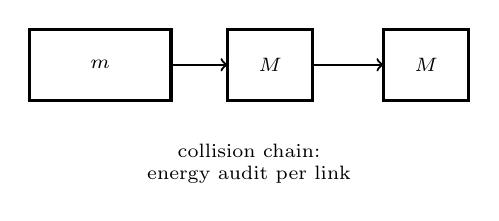
\begin{tikzpicture}[scale=0.9,font=\scriptsize]
\draw[very thick] (-2.4,-0.5) rectangle (-0.4,0.5);
\node at (-1.4,0) {$m$};
\draw[very thick] (0.4,-0.5) rectangle (1.6,0.5);
\node at (1.0,0) {$M$};
\draw[->,thick] (-0.4,0) -- (0.4,0);
\draw[very thick] (2.6,-0.5) rectangle (3.8,0.5);
\node at (3.2,0) {$M$};
\draw[->,thick] (1.6,0) -- (2.6,0);
\node[align=center] at (0.7,-1.4) {collision chain:\\energy audit per link};
\end{tikzpicture}

\caption{The collision chain: audit each link's energy.}
\label{fig:chain}
\end{figure}

\begin{example}[W4: restitution chain audit]\label{ex:w4}
$m_1=1$, $m_2=2$, $v_1=2$, $e=0.5$.
\par\smallskip
\textbf{Strategy.} Restitution formulas + energy before/after.
\begin{solution}
$v_1'=\frac{1-0.5\cdot2-2}{3}(2)/1$... cleaner:
$v_1'=(m_1-em_2)/(m_1+m_2)\,v_1=0$,
$v_2'=(m_1(1+e))/(m_1+m_2)\,v_1=1$\,m/s.
$K_i=2$\,J, $K_f=1$\,J: loss $=1$\,J $=(1-e^{2})\,\frac12\mu v^{2}$
with $\mu=2/3$: $(0.75)(0.5)(2/3)(4)=1.0$\,J. \checkmark
\end{solution}
\textbf{Significance.} The energy loss is entirely fixed by $e$ ---
nothing else to compute.
\end{example}

\begin{figure}[htbp]\centering
\begin{tikzpicture}[scale=0.9,font=\scriptsize]
\draw[very thick] (0,0) circle (1.1);
\draw[very thick] (0,0) circle (0.45);
\draw[thick] (0.45,0) -- (2.2,0.9);
\draw[->,thick,amber] (1.8,0.72) -- (2.2,0.9);
\draw[very thick] (-1.5,-1.1) -- (1.5,-1.1);
\node[align=center] at (0.4,-2.0) {torque about contact:\\roll direction flips at $\cos\theta=r/R$};
\end{tikzpicture}

\caption{The spool: torque about contact flips direction at
$\cos\theta=r/R$.}
\label{fig:spool}
\end{figure}

\begin{example}[W5: the spool's direction flip]\label{ex:w5}
Thread on inner radius $r$ pulled at $\theta$.
\par\smallskip
\textbf{Strategy.} Torque about the instant contact point.
\begin{solution}
$\tau=F(R\cos\theta-r)$: rolls \emph{toward} the pull when
$\cos\theta>r/R$ (small angle), away when steep. At
$\theta=\arccos(r/R)$ it slides without rolling. \checkmark
\end{solution}
\textbf{Significance.} The unintuitive answer falls out of one torque
line --- the classic reason to pick the contact point as pivot.
\end{example}

\begin{example}[W6: meter-stick period]\label{ex:w6}
Pivot at the $20$\,cm mark; CM distance $d=0.3$\,m.
\par\smallskip
\textbf{Strategy.} Physical pendulum $T=2\pi\sqrt{I/mgd}$.
\begin{solution}
$I=I_{cm}+md^{2}=\tfrac1{12}+0.09=0.173$\,kg\,m$^{2}$;
$T=2\pi\sqrt{0.173/2.94}=1.53$\,s --- the code confirms $1.526$\,s.
\checkmark
\end{solution}
\textbf{Significance.} A one-centimeter pivot error is a percent-level
period error --- the measurement design \emph{is} the physics.
\end{example}

\begin{example}[W7: Hohmann $1.5\to2.5R_E$]\label{ex:w7}
\par\smallskip
\textbf{Strategy.} Visc-viva at perigee and apogee.
\begin{solution}
$v_c=6458$\,m/s; burns $762$ and $670$\,m/s; total
$\Delta v=1432$\,m/s. \checkmark
\end{solution}
\textbf{Significance.} Two tangential burns beat any continuous burn
for circular-to-circular transfer.
\end{example}

\begin{example}[W8: satellite capture]\label{ex:w8}
$100$\,kg at the $5$\,m rim of a $5000$\,kg\,m$^{2}$ station at
$0.5$\,rad/s.
\par\smallskip
\textbf{Strategy.} $L$ conserved: $\omega'=L/(I+md^{2})$.
\begin{solution}
$L=5000(0.5)=2500$; $I'=5000+2500=7500$;
$\omega'=0.33$\,rad/s. The ``lost'' $L$ went into the cart's CM ---
which orbits the docking point. \checkmark
\end{solution}
\textbf{Significance.} Angular momentum is never lost; it just moves
into translation you forgot to count.
\end{example}

\begin{figure}[htbp]\centering
\begin{tikzpicture}[scale=0.85,font=\scriptsize]
\draw[very thick,accent] (0,0) circle (1.7);
\draw[very thick,dashed] (-1.7,0) -- (1.7,0);
\foreach \x/\y in {-1.2/0,0/0,1.2/0}{\draw[->,thick,amber] (\x,\y+0.4) -- (\x,\y);}
\node[align=center] at (0,-2.4) {$g(r)=g\,r/R$ inside:\\SHM, $T=84.4$ min};
\end{tikzpicture}

\caption{The tunnel problem: inside a uniform Earth, $g\propto r$
makes it a spring.}
\label{fig:tunnel}
\end{figure}

\begin{example}[W9: tunnel through Earth]\label{ex:w9}
Uniform density: find the transit time to the far side.
\par\smallskip
\textbf{Strategy.} Inside a uniform sphere $g(r)=gr/R$ ---
a Hooke's-law restoring force.
\begin{solution}
$\ddot x=-(g/R)x$: SHM with $T=2\pi\sqrt{R/g}=84.4$\,min; the far
side lands at $T/2=42.2$\,min --- \emph{independent} of which chord
the tunnel takes (same restoring constant). \checkmark
\end{solution}
\textbf{Significance.} 42 minutes to anywhere --- the famous number is
the uniform-density answer, and the sim confirms it.
\end{example}

\begin{example}[W10: sand in the cart]\label{ex:w10}
Sand falls \emph{vertically} at $2$\,kg/s into a $5$\,m/s cart.
\par\smallskip
\textbf{Strategy.} $dp_x/dt=0$ along the track (the sand adds no
horizontal momentum).
\begin{solution}
$Mv=\mathrm{const}$: $v(t)=Mv_0/(M+\dot mt)=250/(50+2t)$.
The cart slows because its mass grows --- no horizontal force needed.
\checkmark
\end{solution}
\textbf{Significance.} ``Missing force'' problems are bookkeeping
problems: the momentum left the cart through the added mass.
\end{example}

\begin{example}[W11: disk axis field]\label{ex:w11}
Charge $\sigma$ on a disk of radius $R$; find $E$ at height $z$.
\par\smallskip
\textbf{Strategy.} Only the $z$-component survives; integrate rings.
\begin{solution}
$dE_z=k\,dq\,z/(r^{2}+z^{2})^{3/2}$;
$E(z)=\frac{\sigma}{2\varepsilon_0}\left(1-\frac{z}{\sqrt{z^{2}+R^{2}}}\right)$.
For $z\gg R$: $E\to kQ/z^{2}$ (point limit). \checkmark
\end{solution}
\textbf{Significance.} Every integration exercise ends with a limit
that should reproduce a familiar answer --- check it.
\end{example}

\begin{example}[W12: induced charges in a shell]\label{ex:w12}
Charge $+q$ sits off-centre inside a neutral shell's cavity.
\par\smallskip
\textbf{Strategy.} Field inside conductor $=0$ forces a surface
accounting.
\begin{solution}
Inner surface: total $-q$ (non-uniform --- it crowds near the charge).
Outer: $+q$ spread \emph{uniformly} if the shell is spherical ---
the exterior field is that of a centered $+q$ regardless of the
cavity's mess. \checkmark
\end{solution}
\textbf{Significance.} The conductor screens details: outside sees
only the total.
\end{example}

\begin{example}[W13: two released charges]\label{ex:w13}
$+1$\,\textmu C each, $10$\,g each, released $10$\,cm apart.
\par\smallskip
\textbf{Strategy.} Energy into \emph{both} kinetic energies.
\begin{solution}
$U_i=kq^{2}/r=0.09$\,J; each gets $mv^{2}/2=0.045$:
$v=3.0$\,m/s each (relative $6.0$). \checkmark
\end{solution}
\textbf{Significance.} Split the energy by mass before computing
speeds --- a common one-body mistake.
\end{example}

\begin{figure}[htbp]\centering
\begin{tikzpicture}[scale=0.9,font=\scriptsize]
\draw[very thick] (-1.6,-0.9) rectangle (-0.6,0.9);
\draw[very thick] (0.6,-0.9) rectangle (1.6,0.9);
\draw[fill=accent!20] (-0.3,-0.9) rectangle (0.6,0.9);
\draw[->,thick,amber] (-0.9,0) -- (-0.4,0);
\node[align=center] at (0,-1.7) {fringing field pulls the\\slab in: $F$ from energy};
\end{tikzpicture}

\caption{The dielectric is pulled in: the fringing field does work
whose account is $U_i-U_f$.}
\label{fig:diel}
\end{figure}

\begin{example}[W14: dielectric pull-in]\label{ex:w14}
Slab slides into an \emph{isolated} capacitor at fixed $Q$.
\par\smallskip
\textbf{Strategy.} $U=Q^{2}/2C$ falls as $C$ grows: the drop is the
field's mechanical work.
\begin{solution}
With fraction $x$ of area filled: $C(x)=(\varepsilon_0A/d)(1+(\kappa-1)x)$;
$W_{\rm field}=U_i-U_f$ is positive --- the field \emph{pulls the slab
in}; the lost energy becomes the slab's kinetic energy (or a hand's
heat). \checkmark
\end{solution}
\textbf{Significance.} Same setup, battery attached instead: the sign
flips --- fixed $V$ means the battery pays. Know which reservoir
you're holding constant.
\end{example}

\begin{example}[W15: the lying voltmeter]\label{ex:w15}
$10$\,k$\Omega$ meter across the $5$\,k leg of a
$10\text{k}+5\text{k}$ divider on $15$\,V.
\par\smallskip
\textbf{Strategy.} The meter joins the lower leg in parallel.
\begin{solution}
$R_{leg}=5\|10=3.33$\,k; reading
$=15\times3.33/13.33=3.75$\,V vs the ideal $5$\,V --- the meter lies
by $25\%$. \checkmark
\end{solution}
\textbf{Significance.} Every measurement perturbs the circuit; the
only question is by how much.
\end{example}

\begin{example}[W16: the RC half-and-half ``paradox'']\label{ex:w16}
Battery $\mathcal E$ charges $C$ through $R$: half the energy always
burns.
\par\smallskip
\textbf{Strategy.} Compute both sides; then ask what $R\to0$ changes.
\begin{solution}
Battery: $\mathcal EI$ integrated $=\mathcal EQ=\mathcal E^{2}C$.
Stored: $\tfrac12C\mathcal E^{2}$. Burned: the other half, always ---
the code prints $0.100=0.050+0.050$. For $R\to0$ the current rings up
with stray inductance and the loss rides out in the ringing (or the
spark): the ``paradox'' dissolves into \emph{where} the half goes,
not \emph{whether} it goes. \checkmark
\end{solution}
\textbf{Significance.} Conservation never has paradoxes; only missing
channels.
\end{example}

\begin{figure}[htbp]\centering
\begin{tikzpicture}[scale=0.9,font=\scriptsize]
\draw[very thick] (-1.8,-1.2) rectangle (1.8,1.2);
\foreach \x in {-1.2,-0.6,0,0.6,1.2}{\node at (\x,0) {$\times$};}
\draw[->,thick,accent] (-1.4,0.8) -- (1.4,0.8) node[right]{$\mathbf E$};
\draw[->,very thick] (-3.0,0) -- (-2.0,0) node[left]{$v$};
\draw[thick,dashed] (-2.0,0) .. controls (0.2,0.1) .. (1.9,0.55);
\draw[thick,dashed] (-2.0,0) .. controls (0.2,-0.1) .. (1.9,-0.55);
\node[align=center] at (0,-1.9) {only $v=E/B$ flies straight};
\end{tikzpicture}

\caption{Crossed fields: only $v=E/B$ passes straight through.}
\label{fig:sel}
\end{figure}

\begin{example}[W17: velocity selector design]\label{ex:w17}
Pass $3\times10^{5}$\,m/s ions in $B=0.01$\,T.
\par\smallskip
\textbf{Strategy.} Undeflected needs $qE=qvB$.
\begin{solution}
$E=vB=3000$\,V/m --- figure~\ref{fig:sel}. Any slower ions curve
down, faster up; the slit keeps only the design speed. \checkmark
\end{solution}
\textbf{Significance.} Crossed fields are a filter: mass
spectrometers, Wien filters, and the beam line's first gate.
\end{example}

\begin{figure}[htbp]\centering
\begin{tikzpicture}[scale=0.9,font=\scriptsize]
\draw[very thick] (-0.8,-1.6) -- (-0.8,1.6);
\draw[very thick] (0.8,-1.6) -- (0.8,1.6);
\draw[very thick,accent] (-0.9,0.4) -- (0.9,0.4);
\foreach \x/\y in {-0.4/0.9,0/0.9,0.4/0.9,-0.4/-0.4,0/-0.4,0.4/-0.4}{\node at (\x,\y) {$\times$};}
\draw[->,thick,amber] (0,0.4) -- (0,-0.3) node[right]{$v$};
\node[align=center] at (0,-2.3) {$v_t=mgR/(B^{2}L^{2})$};
\end{tikzpicture}

\caption{The falling rod: motional EMF current brakes the fall at
$v_t$.}
\label{fig:fallrod}
\end{figure}

\begin{example}[W18: falling rod terminal speed]\label{ex:w18}
Rod $m=0.05$\,kg, $L=0.4$\,m, $R=2\,\Omega$, $B=0.5$\,T on vertical
rails.
\par\smallskip
\textbf{Strategy.} At terminal: $mg=ILB$, or equivalently
$mgv=\mathcal E^{2}/R$.
\begin{solution}
$v_t=mgR/(B^{2}L^{2})=24.5$\,m/s; audit: gravity power
$mgv_t=12.0$\,W $=\mathcal E^{2}/R$ exactly. \checkmark
\end{solution}
\textbf{Significance.} The rod's fall is the generator problem run in
reverse --- same audit.
\end{example}

\begin{example}[W19: the same maths twice]\label{ex:w19}
$L=10$\,mH, $C=1$\,\textmu F.
\par\smallskip
\textbf{Strategy.} $\omega_0=1/\sqrt{LC}$.
\begin{solution}
$\omega_0=10^{4}$\,rad/s, $f=1592$\,Hz --- identical to a
$k=100$\,N/m, $m=1$\,kg oscillator; the map is
$m\leftrightarrow L$, $k\leftrightarrow1/C$. \checkmark
\end{solution}
\textbf{Significance.} Once you've solved the oscillator you've solved
every oscillator --- the circuit is a rebadged spring.
\end{example}

\begin{example}[W20: the design estimate]\label{ex:w20}
$1$\,kW to a $12$\,V load over $0.5\,\Omega$ of line.
\par\smallskip
\textbf{Strategy.} $I^{2}R$ at each voltage.
\begin{solution}
At $12$\,V: $I=83$\,A, loss $=I^{2}R=3.5$\,kW --- the line eats more
than the load gets. Step up to $120$\,V: $I=8.3$\,A, loss
$=35$\,W --- a $100\times$ cut from a $10\times$ boost.
\checkmark
\end{solution}
\textbf{Significance.} Chapter~18's whole story in one estimate:
voltage is the loss-killer.
\end{example}

\section{Common mistakes}\label{sec:ws-mistakes}

\begin{tripwire}[Conservation skipped for integration]
Reaching for $\int F\,dx$ when $E$ is conserved --- always check the
conservation laws first.
\end{tripwire}
\begin{tripwire}[Limits left unchecked]
A formula that fails $\mu\to0$ or $r\to\infty$ is wrong; check the
limit before trusting the algebra.
\end{tripwire}
\begin{tripwire}[One-body answers for two-body problems]
Both charges move, both balls swing --- split the energy first.
\end{tripwire}
\begin{tripwire}[Units carried loosely]
One $v^{2}$ forgotten becomes a factor of $10^{4}$ error; carry units
like cargo.
\end{tripwire}
\begin{tripwire}[``Missing'' momentum mourned]
Momentum isn't lost; it moves into the channel you ignored (the sand,
the station's CM, the radiated half).
\end{tripwire}

\section{Summary}\label{sec:ws-summary}

Twenty problems, one method: units first, limits second, conservation
before integration, audit at the end. The resemblance tags point at the
real contest styles --- F=ma, AP-C, USAPhO, APhO --- and the full
solutions keep the Strategy$\to$Solution$\to$Significance frame.

\begin{wins}[Definition of done]
You can now: pick the right conservation law in under a minute, find a
boundary before solving a friction problem, split energies across
bodies, and audit every numeric answer against an order of magnitude.
\end{wins}

\chapternotes{%
Problems are original; the resemblance tags map the genre only. Contest
habits distilled from F=ma past exams \cite{aapt} and the Krotov/Gnädig
problem tradition; the numeric checks come from
\texttt{code/ch19\_workshop\_checks.py}.}

\begin{rulebox}[{Watch instead}]
\begin{enumerate}
\item \emph{US F=ma Physics Olympiad 2025, First Round solutions} ---
Handy Olympiad Physicist, 37:36, \url{https://youtu.be/7pW4zGW0iLQ}
--- the genre these problems mimic, worked at speed (accessed
2026-10-11).
\end{enumerate}
\end{rulebox}

\section*{Further reading}
\addcontentsline{toc}{section}{Further reading}

\begin{itemize}
\item AAPT, \emph{F=ma and USAPhO past exams} --- the real thing, all
years: verified 2026-10-11 at
\url{https://www.aapt.org/physicsteam/2025/pastexams.cfm}.
\item AAPT \emph{U.S. Physics Team} hub --- \url{https://aapt.org}
(verified 2026-10-11).
\item A.~Krotov et al., \emph{Aptitude Test Problems in Physics} ---
the hard-problem tradition (in print).
\item P.~Gn\"adig, G.~Honyek, K.~Riley, \emph{200 Puzzling Physics
Problems} --- problems with the same audit habit (in print).
\item D.~Morin, \emph{Introduction to Classical Mechanics} chs.~1--8
--- the mechanics half at olympiad depth (in print).
\item Art of Problem Solving physics forums --- community solutions and
variants: at \url{https://artofproblemsolving.com} (verified
2026-10-11).
\end{itemize}
